Um die Genauigkeit des entwickelten Müdigkeitsdetektors einschätzen zu können, muss dieser evaluiert werden. Da verschiedene Verfahren und Metriken in die Abläufe involviert sind, ist nicht nur eine gesamtheitliche, sondern auch eine granulare Bewertung einzelner Stufen als sinnvoll anzusehen. 

\subsection{Das Interface}
\label{ssec:interface}

Die App bietet eine Benutzeroberfläche mit verschiedenen Bildschirmen, wie in der Abbildung \ref{fig:screens} zu erkennen ist.

\begin{figure}[h]
	\centering
	\begin{subfigure}[b]{0.22\textwidth}
		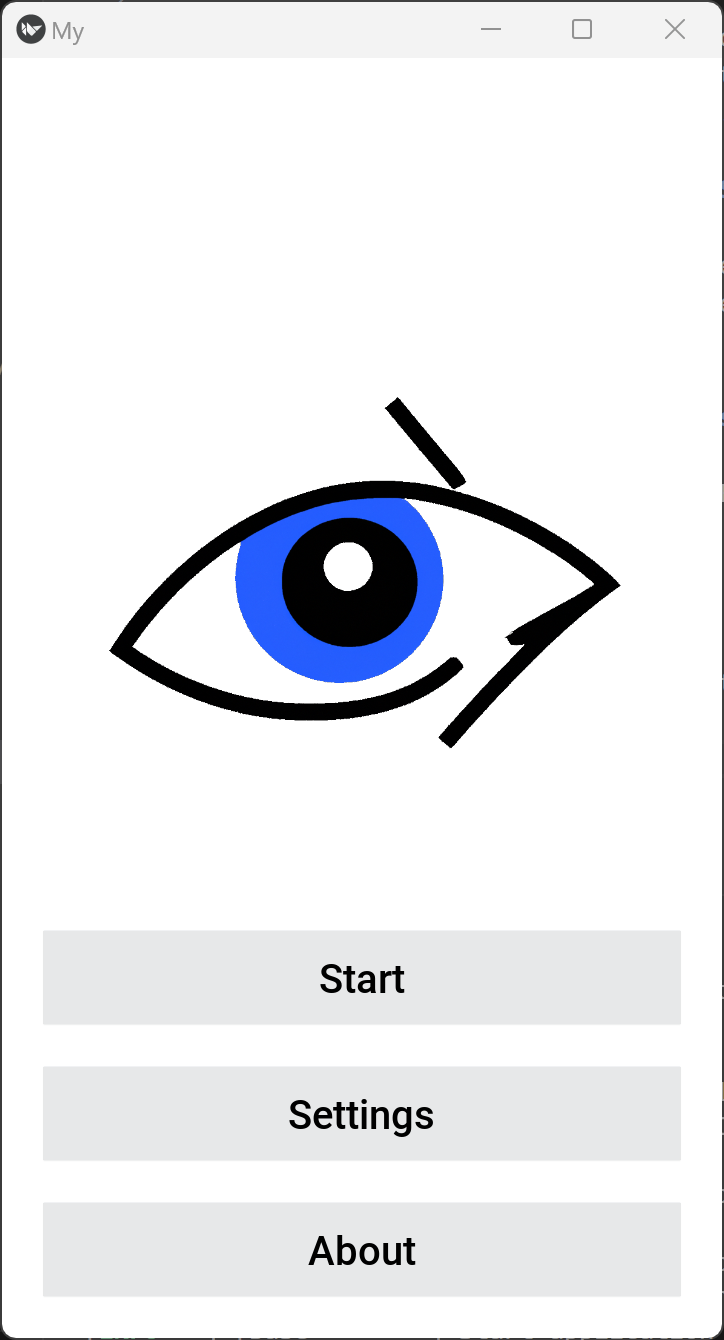
\includegraphics[width=\linewidth]{images/mainscreen.png}
		\caption{Startseite}
		\label{fig:mainscreen}
	\end{subfigure}
	\hfill
	\begin{subfigure}[b]{0.22\textwidth}
		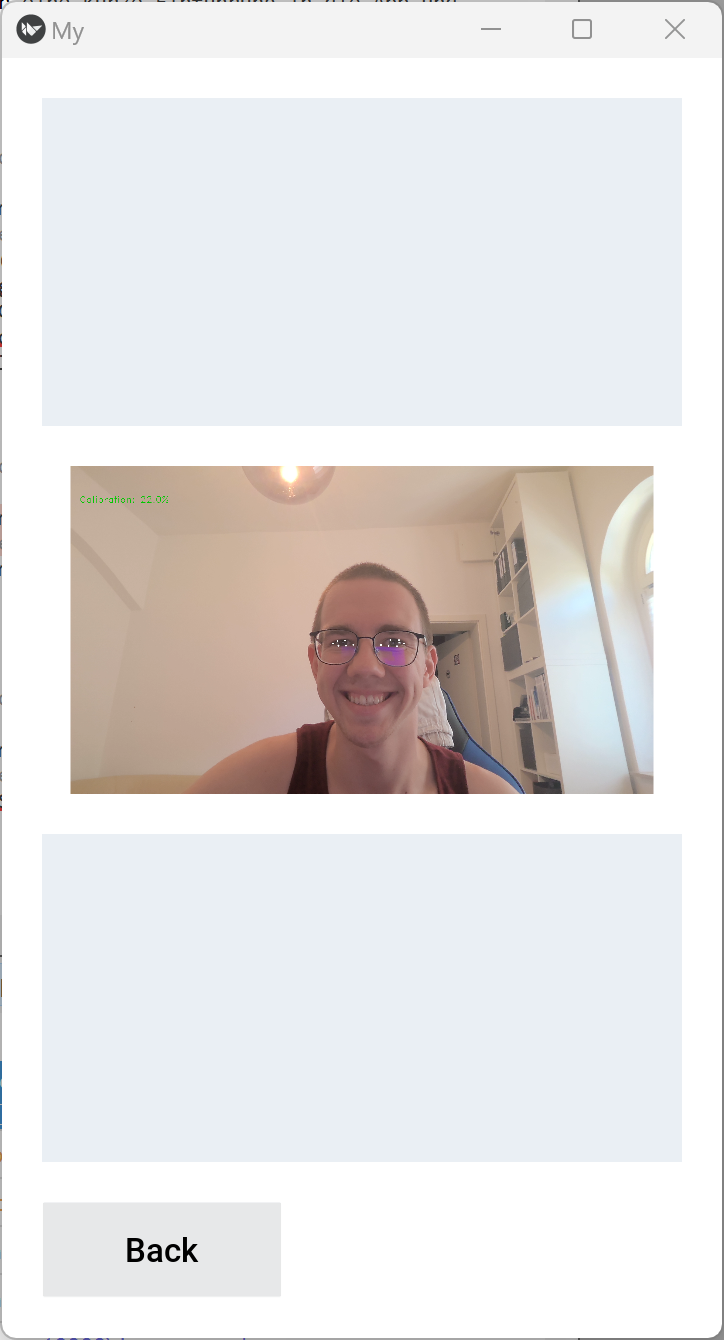
\includegraphics[width=\linewidth]{images/detectionscreen.png}
		\caption{Detektion}
		\label{fig:detectionscreen}
	\end{subfigure}
	\hfill
	\begin{subfigure}[b]{0.22\textwidth}
		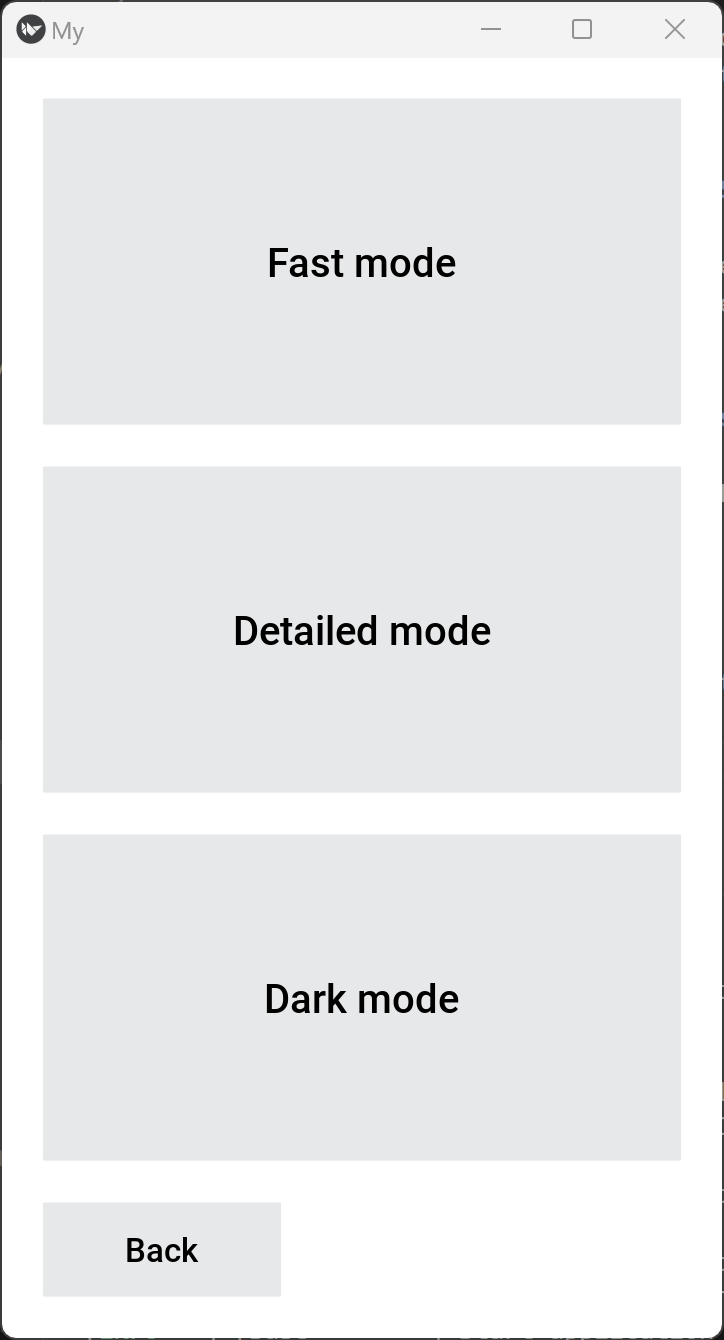
\includegraphics[width=\linewidth]{images/settingscreen.png}
		\caption{Einstellungsseite}
		\label{fig:settingscreen}
	\end{subfigure}
	\hfill
	\begin{subfigure}[b]{0.22\textwidth}
		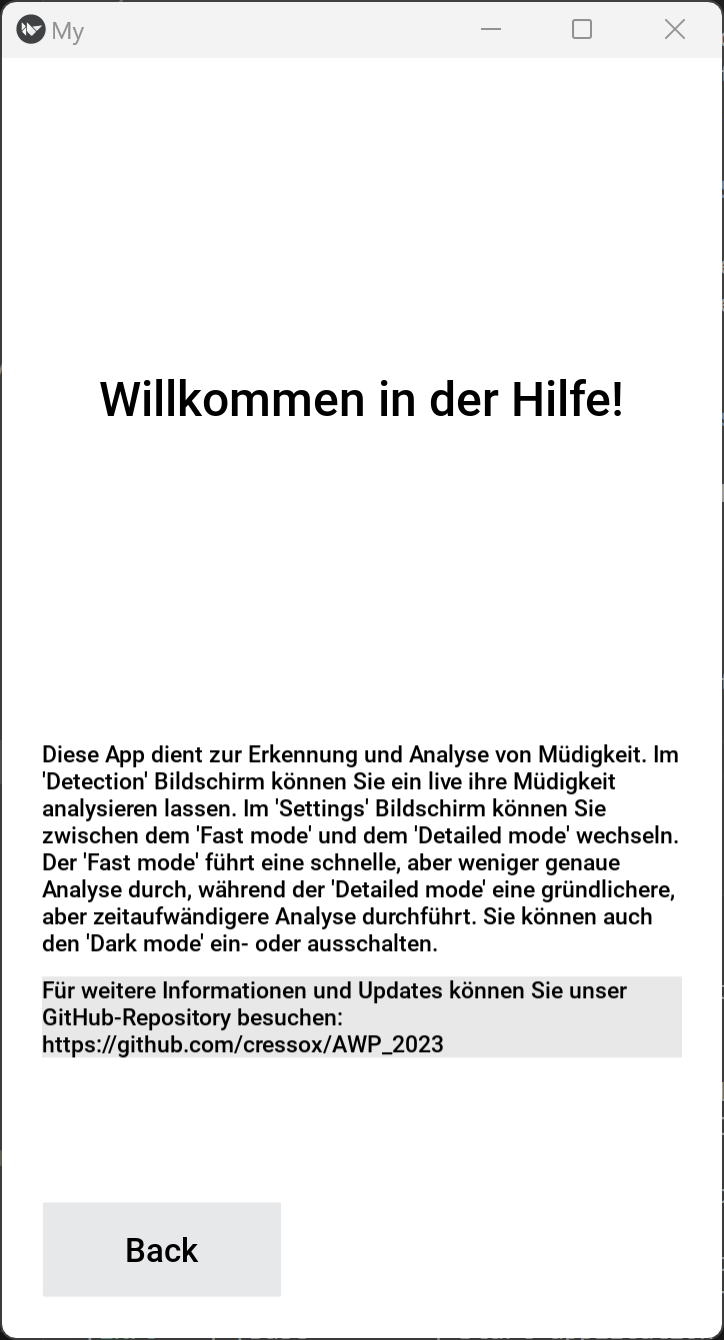
\includegraphics[width=\linewidth]{images/helpscreen.png}
		\caption{Hilfebereich}
		\label{fig:helpscreen}
	\end{subfigure}
    \caption{Verschiedene Screenshots aus der Anwendung.}
    \label{fig:screens}
\end{figure}

In Abbildung \ref{fig:mainscreen} ist der Einstiegsbildschirm der App zu sehen. Hier erhalten Benutzer eine kurze Einführung in die App und können die Müdigkeitserkennung starten oder auf die Einstellungen zugreifen. Die eigentliche Müdigkeitserkennung findet im Erkennungsbildschirm (Abbildung \ref{fig:detectionscreen}) statt, wo erkannte Gesichtsmerkmale wie die Augen markiert werden. Bei Erkennung von Müdigkeitsmerkmalen kann die App Warnungen anzeigen oder Alarmtöne abspielen. Im Einstellungsbildschirm (Abbildung \ref{fig:settingscreen}) können Benutzer verschiedene Einstellungen für die Benutzeroberfläche anpassen. Der Hilfebildschirm (Abbildung \ref{fig:helpscreen}) bietet detaillierte Informationen zur Verwendung der App und ihrer Funktionen.

Grundsätzlich sind wir mit dem Layout zufrieden, da es Minimalismus und Nutzbarkeit vereint. Der gesamte Funktionsumfang wird von der App abgedeckt und dem Nutzer zur Verfügung gestellt. Hierbei ist die Bedienung selbsterklärend und zielführend, ohne die potenziellen Nutzer vor Schwierigkeiten der Orientierung zu stellen. Wie in Abschnitt \ref{ssec:lessonslearned} bereits erwähnt, hätte mehr Zeit in die Möglichkeiten der Entwicklung investiert werden können, somit hätte das Design noch interaktiver und flexibler sein können.

\subsection{Selbsttest zu Metriken und Frameworks}
\label{subsec:selftest}
Zur Evaluation verschiedener Schwellwerte zur Blinzeldetektion und Frameworks wurde einen Selbsttest im Wachzustand durchgeführt, wobei zu zweit in einer alltäglichen Arbeitsumgebung mit natürlicher Beleuchtung über die interne Webcam des eigenen Laptops das Programm circa eine Minute lang ausgeführt wurde. Von diesen Versuchen entnahmen wir die selbstgezählte reale und die detektierte Anzahl der Blinzelschläge in diesem Zeitraum für verschiedene Parametervoreinstellungen. Zusätzlich führten wir dies für zwei verschiedene Frameworks aus, um durch Selbsttests herauszufinden, welches für unseren Anwendungsbereich geeigneter ist. Für Proband 1 ist in Tabelle \ref{table:selbsttest} zu erkennen, dass MediaPipe im Durchschnitt eine signifikant bessere Detektionsrate aufweisen kann als Dlib. Hierbei ist es wichtig, dass weder zu viele noch zu wenig Blinzelschläge detektiert werden. Da keine Toleranz für Fehldetektionen geplant war, ist dieser Wert zu optimieren. Für Probanden 2 sind ähnliche Ergebnisse zu verzeichnen, eine fehlerfreie Erkennung kann auch hier nur MediaPipe liefern. Jedoch ist zu bemerken, dass für diese Versuchsperson die optimale Detektion nur bei einem kleineren Schwellwert des EAR-Wertes gegeben ist. Zu begründen ist dies durch die generellen Unterschiede in Individuen sowie die persönliche Form und Anatomie des Auges. Für jede Person ist der EAR-Wert im geöffneten Zustand verschieden, ein kleinerer Wert tendiert dazu, dass bei einem vergleichsweise hohen Schwellwert einige Blinzelschläge fälschlicherweise erkannt werden, da der Schwellwert bereits ohne ein Schließen des Auges unterschritten wird. Dies ist auch in dem Test aufgefallen, so wurden für einige Kombinationen zu viele Blinzelschläge detektiert, weshalb der Detektor nicht vertrauenswürdig wäre. Ein zu kleiner Schwellwert resultiert jedoch darin, dass aufgrund der möglicherweise geringen Framerate der Videos ein Blinzeln nicht erkannt wird, wenn nicht zufälligerweise ein Bild bei der vollständigen Schließung des Auges aufgenommen wird. Nach Beachtung dieser Zusammenhänge und Auswertung der Tabelle des Selbsttest (Tabelle \ref{table:selbsttest}) ist der Entschluss zu ziehen, dass die Benutzung von MediaPipe als Framework das geeignetere Mittel ist. Weiterhin stellte sich der Schwellwert für die Blinzeldetektion von 0.16 als passend heraus, da dieser verschiedene Probleme minimiert. Für diesen Wert wurde die höchste Genauigkeit erreicht, da sowohl die Anzahl der falschpositiven als auch falschnegativen Werte für das ausgewählte Framework gleich Null ist. Somit ist zu sagen, dass die implementierte Detektion verlässlich und genau arbeitet. 

\begin{table}[!htp]\centering
	\scriptsize
	\begin{tabular}{lrrrrr}%\toprule
		&\multicolumn{4}{c}{\textbf{Detektierte/reale Blinzelschläge}} \\\cmidrule{2-5}
		&\multicolumn{2}{c}{\textbf{Proband 1}} &\multicolumn{2}{c}{\textbf{Proband 2}} \\\cmidrule{2-5}
		\textbf{Blink Threshold} &\textbf{Dlib} &\textbf{MediaPipe} &\textbf{Dlib} &\textbf{MediaPipe} \\\midrule
		\multirow{2}{*}{0.16} &33/43 &45/45 &54/53 &54/54 \\
		&39/53 &58/58 &49/47 &61/61 \\
		\multirow{2}{*}{0.18} &38/48 &60/60 &49/47 &61/50 \\
		&33/52 &60/53 &57/52 &42/41 \\
		\multirow{2}{*}{0.20} &50/52 &64/64 &65/44 &60/37 \\
		&47/53 &57/57 &57/49 &70/45 \\
		& & & & \\
		\textbf{$\varnothing$ EAR} &0.32 &0.295 &0.259 &0.252 \\
		& & & & \\
		\textbf{$\varnothing$ PERCLOS} &0.08 &0.063 &0.109 &0.107 \\
		%\bottomrule
	\end{tabular}
	\caption{Selbsttest zu verschiedenen Schwellwerten und Frameworks}\label{table:selbsttest}
\end{table}

Neben der Anzahl der Blinzelschläge wurden zusätzlich die durchschnittlichen EAR- und PERCLOS-Werte betrachtet, um eventuelle Zusammenhänge nachvollziehen zu können. Hierbei ist deutlich zu entnehmen, dass der EAR-Wert für Proband 2 deutlich kleiner und der PERCLOS-Wert deutlich größer als die des Probanden 1 sind. Dies spiegelt genau die Zusammenhänge der Metriken und der verschiedenen geeigneten Schwellwerts wider, da für Proband 2 ein kleinerer Schwellwert besser geeignet ist, was auf ein generell schwächer geöffnetes Auge hinweist. Dies würde in einem geringeren EAR-Wert resultieren, was die Daten verifizieren. Weiterhin sollte der PERCLOS-Wert höher sein, je größer die Anzahl an Blinzelschlägen oder je länger die Blinzeldauer pro Zeitspanne ist, da der Anteil, in dem die Augen geschlossen sind, größer ist. Unsere Beobachtungen stimmen mit diesem Verhalten überein, für Proband 1 wurde ein kleinerer Wert als für Proband 2 ermittelt.

\subsection{Vergleich der Klassifikatoren}
\label{subsec:classificatorcomparison}
Wie in der Theorie im Abschnitt \ref{sec:classification} zur Klassifikation beschrieben, wurden verschiedene Klassifikatoren getestet, um den am besten geeigneten für unsere Anwendung zu ermitteln. Dabei haben wir sowohl den Fall mit zwei Klassen (müde/wach) als auch den mit drei Klassen (müde/fraglich/wach) getestet. Die Metriken, die wir verwendet haben, wurden in Abschnitt \ref{sec:classificationmetrics} vorgestellt.

\begin{table}[!htp]
	\centering
	\scriptsize
	\begin{tabular}{lcccc}%\toprule
		\textbf{Klassifikator} & \textbf{F1-Score} & \textbf{Recall} & \textbf{Precision} & \textbf{Accuracy} \\\midrule
		\textbf{KNN Klassifikator mit k = 3} & 0.743962 & 0.758621 & 0.801724 & 0.680542 \\
		\textbf{Logistische Regression} & 0.663643 & 0.689655 & 0.671121 & 0.602709 \\
		\textbf{Support Vector Machine} & 0.552622 & 0.62069 & 0.79454 & 0.489655 \\
	\end{tabular}
	\caption{Ergebnisse der drei verglichenen Klassifikatoren über die vorgestellten Metriken für die drei Klassen wach, fraglich und müde.}
	\label{table:threeclassificator}
\end{table}


Die Trainingsdaten für die Klassifikatoren bestehen aus den berechneten Feature-Vektoren, die aus den Videos des verwendeten Datensatzes gewonnen wurden. Insgesamt hatten wir 144 Feature-Vektoren, davon jeweils 48 für die Zustände \glqq müde\grqq{}, \glqq fraglich\grqq{} und \glqq wach\grqq{}, jeweils einmal für jeden Probanden. Um die Feature-Vektoren zu erstellen, haben wir die ersten sechs Minuten jedes Videos für die Kalibrierung genutzt. Die Aufteilung in Test- und Trainingsdatensätze erfolgte zufällig über die 144 Feature-Vektoren, unabhängig von der Person. Durch eine fünf-fache Crossvalidierung haben wir immer 20 Prozent als Test- und 80 Prozent als Trainingsdaten verwendet. Die Werte für \glqq fraglich\grqq{} und \glqq müde\grqq{} wurden ins Verhältnis zu den Wachwerten gesetzt, und danach wurden die Klassifikatoren trainiert. Dies führte dazu, dass für jedes Feature ein Wach-Wert von 1 vorlag, was die Ergebnisse der Klassifikatoren beeinflusste und bessere Ergebnisse für die verwendeten Metriken lieferte, da alle Testdaten für \glqq wach\grqq{} richtig klassifiziert wurden. Trotzdem ergibt die Klassifikation Sinn, da sie eine sinnvolle Trennung zwischen den Klassen ermöglicht und eine signifikante Abweichung von Werten der Klasse \glqq wach\grqq{} für die Klassifikation von \glqq fraglich\grqq{} und \glqq müde\grqq{} aufzeigt.

\begin{table}
    \centering
    \scriptsize
    \begin{tabular}{llll}
    \multicolumn{4}{c}{\textbf{KNN Klassifikator mit k=3}} \\
    & \textbf{vorhergesagt wach} & \textbf{vorhergesagt fraglich} & \textbf{vorhergesagt müde} \\ \hline
    \textbf{Wahr wach} & 13 & 0 & 0 \\ 
    \textbf{Wahr fraglich} & 0 & 3 & 6 \\ 
    \textbf{Wahr müde} & 0 & 1 & 6 \\ 
    \end{tabular}
    
    \vspace{0.5cm} % Vertikaler Abstand zwischen den Tabellen
    
    \begin{tabular}{llll}

    \multicolumn{4}{c}{\textbf{Support Vector Machine}} \\ 
    & \textbf{vorhergesagt wach} & \textbf{vorhergesagt fraglich} & \textbf{vorhergesagt müde} \\ \hline
    \textbf{Wahr wach} & 13 & 0 & 0 \\ 
    \textbf{Wahr fraglich} & 8 & 1 & 0 \\ 
    \textbf{Wahr müde} & 3 & 0 & 4 \\ 
    \end{tabular}
    
    \vspace{0.5cm} % Vertikaler Abstand zwischen den Tabellen
    
    \begin{tabular}{llll}

    \multicolumn{4}{c}{\textbf{Logistische Regression}} \\ 
    & \textbf{vorhergesagt wach} & \textbf{vorhergesagt fraglich} & \textbf{vorhergesagt müde} \\ \hline
    \textbf{Wahr wach} & 13 & 0 & 0 \\ 
    \textbf{Wahr fraglich} & 2 & 3 & 4 \\ 
    \textbf{Wahr müde} & 1 & 2 & 4 \\ 
    \end{tabular}

\caption{Confusion Matritzen für die drei Klassifikatoren für die drei Klassen wach, fraglich und müde.}
\label{table:confusionmatrixthreeclasses}
\end{table}



Die Ergebnisse zeigen im direkten Vergleich der Klassifikatoren für drei Klassen in Tabelle \ref{table:threeclassificator}:

\begin{itemize}
\item Alle Metriken sind bei dem KNN-Klassifikator am besten, wobei die Accuracy und die Precision die höchsten Werte aufweisen.
\item Bei der Logistic Regression ist die Accuracy höher (0.60) als bei der SVM (0.49), jedoch ist die Precision niedriger (0.67 gegenüber 0.79).
\item Der F1 Score und der Recall sind ebenfalls beim KNN-Klassifikator am höchsten.
\end{itemize}

Ein Blick auf die Confusion Matrizen eines Durchlaufs der Crossvalidierung lohnt sich (siehe Tabelle \ref{table:confusionmatrixthreeclasses}, insbesondere wenn man bedenkt, dass eine Fehlklassifikation von \glqq wach\grqq{} oder \glqq fraglich\grqq{} als \glqq müde\grqq{} in unserem Fall weniger problematisch ist als die Fehlklassifikation von \glqq müde\grqq{} als \glqq wach\grqq{} oder \glqq fraglich\grqq{}. Da wir vor Sekundenschlaf warnen möchten, ist eine frühzeitige fehlerhafte Warnung weniger problematisch, natürlich unter der Berücksichtigung, dass zu viele Warnungen als nicht zielgerichtet empfunden werden könnten. Die Confusion Matrix für den KNN-Klassifikator zeigt beispielsweise, dass sechs \glqq fragliche\grqq{} Videos als \glqq müde\grqq{} klassifiziert wurden, während bei der SVM und der Logistischen Regression eine größere Streuung zu sehen ist: bei der SVM wurden acht Videos als \glqq wach\grqq{} statt \glqq fraglich\grqq{} klassifiziert, und bei der logistischen Regression zwei als \glqq wach\grqq{} statt \glqq fraglich\grqq{}. Dies ist in unserem Fall ungünstig. Der KNN-Klassifikator hat keine Videos fehlerhaft als \glqq wach\grqq{} klassifiziert, sondern lediglich ein Video als \glqq fraglich\grqq{} anstatt \glqq müde\grqq{}. Daher zeigt sich der KNN-Klassifikator als die beste Wahl zur Detektion von Müdigkeit.

\begin{table}
    \centering
    \begin{tabular}{lllll}

        \textbf{Klassifikator} & \textbf{F1-Score} & \textbf{Recall} & \textbf{Precision} & \textbf{Accuracy} \\ \hline
        \textbf{KNN Klassifikator mit k = 3} & 1 & 1 & 1 & 0.947368 \\ 
        \textbf{Logistische Regression} & 1 & 1 & 1 & 0.904094 \\ 
        \textbf{Support Vector Machine} & 0.88797 & 0.894737 & 0.908772 & 0.712865 \\ 
    \end{tabular}
\caption{Ergebnisse der drei verglichenen Klassifikatoren über die vorgestellten Metriken für die zwei Klassen wach und müde.}
\label{table:twoclassificator}
\end{table}

Der Vergleich von zwei Klassen führte aufgrund der in Relation gesetzten Werte zu einem noch besseren Ergebnis und dennoch konnte auch hier eine klare Trennung erreicht werden. Wie in Tabelle \ref{table:twoclassificator} haben die logistische Regression und der KNN-Klassifikator beide sehr gut abgeschnitten, wobei die Accuracy beim KNN-Klassifikator höher war als bei der logistischen Regression. Dies bedeutet, dass der KNN-Klassifikator in allen Durchläufen eine bessere Klassifikation durchgeführt hat. Ein Beispiel aus einem Kreuzvalidierungsdurchlauf zeigt, dass der KNN-Klassifikator und die logistische Regression in diesem Fall alles richtig klassifiziert haben (siehe Tabelle \ref{table:confusionmatrixtwoclasses}), wie auch die Werte von 1 bei den F1-, Recall- und Precision-Werten in Tabelle \ref{table:twoclassificator} zeigen. Die SVM hat in diesem Fall jedoch zwei Werte falsch klassifiziert. Hier ist der Accuracy Score am ausschlaggebendsten.


\begin{table}
    \centering
    \begin{tabular}{lll}

    \multicolumn{3}{c}{\textbf{KNN Klassifikator mit k=3}}\\
    & \textbf{vorhergesagt wach} & \textbf{vorhergesagt müde} \\ \hline
    \textbf{Wahr wach} & 13 & 0 \\ 
    \textbf{Wahr müde} & 0 & 6 \\ 
    \end{tabular}
    
    \vspace{0.5cm} % Vertikaler Abstand zwischen den Tabellen
    
    \begin{tabular}{lll}
    
    \multicolumn{3}{c}{\textbf{Support Vector Machine}}\\
    & vorhergesagt wach & vorhergesagt müde \\ \hline
    \textbf{Wahr wach} & 13 & 0 \\ 
   \textbf{ Wahr müde} & 0 & 6 \\ 
    \end{tabular}
    
    \vspace{0.5cm} % Vertikaler Abstand zwischen den Tabellen
    
    \begin{tabular}{lll}
    
    \multicolumn{3}{c}{\textbf{Logistische Regression}} \\ 
    & \textbf{vorhergesagt wach} & \textbf{vorhergesagt müde} \\ \hline
   \textbf{ Wahr wach} & 13 & 0 \\ 
    \textbf{Wahr müde }& 2 & 4 \\ 
    \end{tabular}
\caption{Confusion Matritzen für die drei Klassifikatoren für die zwei Klassen wach und müde.}
\label{table:confusionmatrixtwoclasses}
\end{table}

\subsection{Müdigkeitserkennung in der Anwendung}
\label{subsec:runningdrowsinessdetection}

In der Anwendung erfolgt die Kalibrierung des Wachzustands in den ersten 60 Sekunden, in denen die Feature-Vektoren für den Wachzustand berechnet werden. Es sei denn, die Person dreht sich zur Seite oder bewegt sich aus dem Blickfeld, was die Kalibrierung anhält. Wenn die Person für mehr als drei Sekunden nicht nach vorne schaut, ertönt ein Warnton, um den Fahrer zur Konzentration auf die Straße und erhöhten Aufmerksamkeit aufzufordern, da Ablenkung ebenfalls zu Unfällen führen kann.

Nach der Kalibrierung wird für jedes Einzelbild der aktuelle Feature-Vektor neu berechnet und ins Verhältnis zu den Wachwerten gesetzt. Wenn der KNN-Klassifikator eine signifikante Abweichung von den Wachwerten feststellt, ändert sich die Farbe um das Video herum, zuerst zu Orange (\glqq fraglich\grqq{}) und anschließend zu Rot (\glqq müde\grqq{}). Um abrupte Änderungen, wie sie in unseren Tests auftraten, auszugleichen, wird der Medianwert (wach/fraglich/müde) der letzten 60 Sekunden als maßgebend betrachtet.

Wenn eine Person über einen längeren Zeitraum im müden Zustand verbleibt, erfolgt eine wiederholte Warnung. Dies geschieht alle zehn Sekunden, um eine angemessene Häufigkeit sicherzustellen. Zusätzlich wird eine Warnung ausgegeben, wenn eine Person unabhängig von ihrem Status die Augen zu lange geschlossen hält, in unserem Fall beträgt dies genau zwei Sekunden.

Unsere Tests haben gezeigt, dass unser Müdigkeitsdetektionskonzept eine solide Grundlage bietet, jedoch die verschiedenen Parameter nicht für jede Person optimal sind. Es gibt auch feststellbare Abweichungen in Bezug auf den Zeitpunkt, zu dem Warnungen ausgegeben werden, was vermutlich auf gelegentliche Berechnungsfehler zurückzuführen ist. Dies sind normale Schwankungen, die in Zukunft genauer betrachtet werden sollten. Trotzdem funktioniert der Übergang zwischen den verschiedenen Zuständen, auch wenn man sich in manchen Situationen nur sehr kurz im Zustand \glqq fraglich\grqq{} befindet.


